%++++++++++++++++++++++++++++++++++++++++
% Don't modify this section unless you know what you're doing!
\documentclass[a4paper,12pt]{article}
\usepackage{listings} % code blocks
\usepackage{tabularx} % extra features for tabular environment
\usepackage{amsmath}  % improve math presentation
\usepackage{graphicx} % takes care of graphic including machinery
\usepackage{subcaption} % necessary for subfigures
\usepackage{float}
\usepackage[margin=3.0cm,a4paper]{geometry} % decreases margins
%\usepackage{cite} % takes care of citations
%\usepackage[final]{hyperref} % adds hyper links inside the generated pdf file
%++++++++++++++++++++++++++++++++++++++++

\setlength{\parindent}{0pt}
\usepackage{hyperref}

\begin{document}

\title{Deep Learning Lab \\ Exercise 02 }
\author{Megan Klaiber}
\date{\today}
\maketitle
\section{Introduction}
In this exercise a multi-layer perceptron (MLP) will be implemented to classify the handwritten MNIST digits. Different hyperparameters are tested to achieve a good result on a test set.\\
The implementation of the MLP is done according to the given framing.


\section{Neural Network}
\subsection{Implementation}
For the implementation of an MLP three activation functions can be used in the hidden layers: Sigmoid, Tanh and Relu. Softmax and linear are available for the output layer. Gradient descent (GD) and stochastic gradient descent (SGD) are implemented for optimization.

\subsection{Result}\label{result}
The resulting model with the best performance is a neural network with one hidden layer containing 220 units. This layer utilizes a Relu activation function. For the output layer the softmax function was used. The network was trained with 50.000 images and validated on 10.000 images. With the following hyperparameters the error on the validation set converges to 1,86\%:

\begin{itemize}
	\item learning rate: 0.15
	\item epochs: 30
	\item batch size: 30
	\item optimizer: stochastic gradient descent
\end{itemize}

\autoref{fig:train_valid_error} shows the error on the training and validation set during the training. With a trained model on the full dataset (training and validation set) a test error of 1.73\% on unseen test data was achieved.

\begin{figure}[H]
  \centering 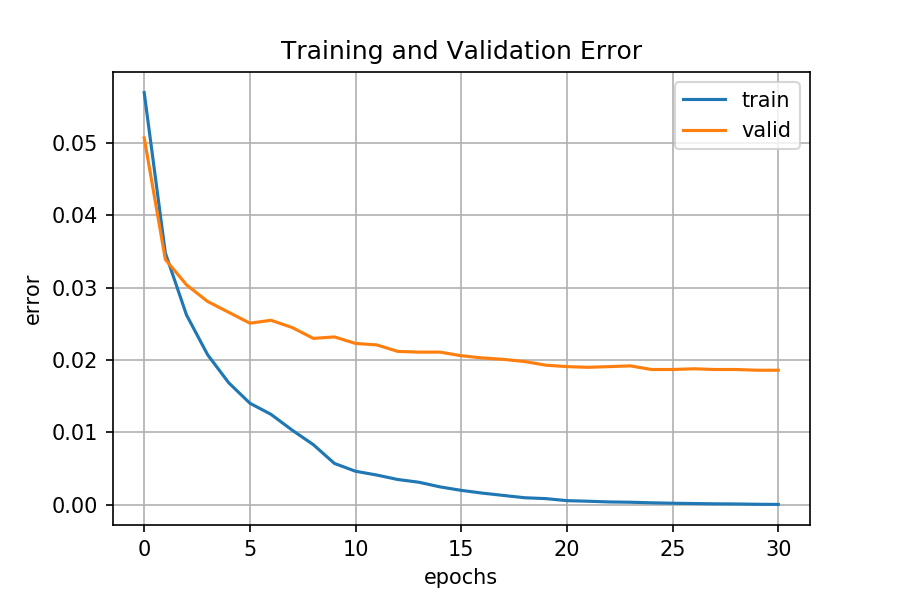
\includegraphics[width=11.70cm, height=7.9cm]{plots/train_valid_error.png}
  \caption{
    \label{fig:train_valid_error}
    Change of training and validation error while training epochs of MLP on MNIST dataset. MLP has one hidden layer with 220 units and ReLu activation. Optimization with SGD used a learning rate of 0.15 and batches of 30 images.
  }
\end{figure}

\subsection{Optimization}\label{opt}
To see how different optimizers influence the training, gradient descent and stochastic gradient descent were compared. Therefore the settings from \autoref{result} are used. \autoref{fig:sgd_gd_error.png} compares the training error for the two optimizers. It implies that gradient descent converges slower than stochastic gradient descent.


\begin{figure}[H]
	\centering 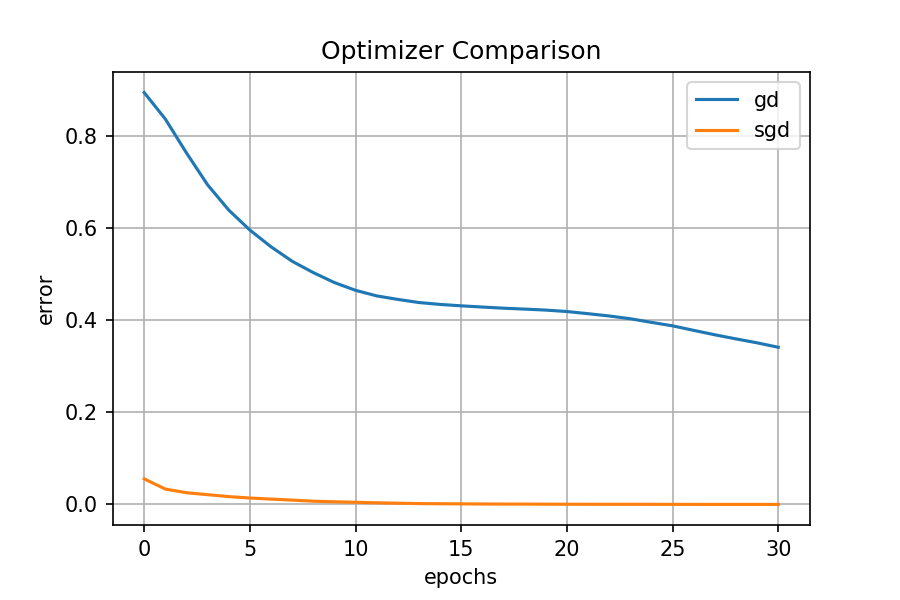
\includegraphics[width=11.7cm, height=7.9cm]{plots/sgd_gd_error.png}
	\caption{
		\label{fig:sgd_gd_error.png}
		Change of training error with gradient descent and stochastic gradient descent as optimizers.
	}
\end{figure}

\section{Conclusion}
With this exercise you can see that a simple MLP achieves good results on the MNIST dataset. In \autoref{opt} you can see that the right optimization method is important for the training procedure. In addition it is possible to achive better results if you add regularization techniques.

\end{document}
